\documentclass[conference]{IEEEtran}
\IEEEoverridecommandlockouts
% The preceding line is only needed to identify funding in the first footnote. If that is unneeded, please comment it out.
\usepackage{cite}
\usepackage{amsmath,amssymb,amsfonts}
\usepackage{algorithmic}
\usepackage{graphicx}
\usepackage{textcomp}
\usepackage{xcolor}
\usepackage{tabularx}
\def\BibTeX{{\rm B\kern-.05em{\sc i\kern-.025em b}\kern-.08em
    T\kern-.1667em\lower.7ex\hbox{E}\kern-.125emX}}
\begin{document}

\title{Reinforcement Learning and Agent Based Modeling for Socio-Ecological Systems Management : A Systematic Review}

\author{\IEEEauthorblockN{Cheikhou Akhmed Kane}
\IEEEauthorblockA{\textit{dept. name of organization (of Aff.)} \\
\textit{name of organization (of Aff.)}\\
City, Country \\
email address or ORCID}
\and
\IEEEauthorblockN{Samba Diaw}
\IEEEauthorblockA{\textit{dept. name of organization (of Aff.)} \\
\textit{name of organization (of Aff.)}\\
City, Country \\
email address or ORCID}
\and
\IEEEauthorblockN{Mandicou Ba}
\IEEEauthorblockA{\textit{dept. name of organization (of Aff.)} \\
\textit{name of organization (of Aff.)}\\
City, Country \\
email address or ORCID}
\and
\IEEEauthorblockN{Alassane Bah}
\IEEEauthorblockA{\textit{dept. name of organization (of Aff.)} \\
\textit{name of organization (of Aff.)}\\
City, Country \\
email address or ORCID}
}

\maketitle

\begin{abstract}
The sustainable management of complex Socio-Ecological Systems (SES) requires models that can capture both decentralized human behaviors and optimal long-term policies. The coupling of Agent-Based Models (ABM) and Multi-Agent Reinforcement Learning (MARL) is a relevant paradigm, but "full MARL" approaches often face critical barriers in computational cost and scalability. This paper presents a systematic review (PRISMA) to map the state-of-the-art of this coupling, focusing on applications in environmental sustainability.

A multi-faceted query strategy—targeting core technology (Q1), thematic applications (Q2), and hierarchical architectures (Q3)—was deployed across general (e.g., Scopus, Web of Science) and specialized (e.g., IEEE Xplore, ACM) databases, filtered from 2017 to capture the modern Deep MARL era.

Our synthesis of the resulting corpus identifies key research gaps, particularly in model validation and scalability. Based on this analysis, we conclude that hierarchical architectures emerge as a highly promising research direction. These models, which can combine high-level learning agents with simpler behavioral rules, appear particularly suited to overcoming critical barriers in real-world deployments, such as scalability and effective application in data-poor environments.
\end{abstract}

\begin{IEEEkeywords}
Multi-Agent Reinforcement Learning (MARL), Agent-Based Modeling (ABM), Socio-Ecological Systems (SES)
\end{IEEEkeywords}

\section{Introduction}
The modeling and sustainable management of Socio-Ecological Systems (SES) constitute significant scientific challenges. These systems, characterized by the coexistence of biophysical dynamics and human behaviors, exhibit inherent complexity, non-linear interactions, and actor heterogeneity, making the prediction of outcomes and the design of optimal interventions particularly arduous.

In response to this challenge, the bottom-up paradigm is frequently employed over traditional top-down models. Within this paradigm, Agent-Based Modeling (ABM) has become a prevalent simulation tool. While conceptually close to Multi-Agent Systems (MAS), a broader field within computer science, ABMs are specifically valued in social and ecological sciences for their capacity to simulate decentralized interactions and observe the emergence of collective behaviors.

However, traditional ABMs often face limitations in modeling complex and adaptive human decision-making under uncertainty. It is in this context that Reinforcement Learning (RL), and more specifically Multi-Agent Reinforcement Learning (MARL), offers a relevant methodological framework. MARL provides the formal tools for agents to learn decision-making policies through \textit{trial-and-error} interaction with dynamic environments.

This coupling of ABM and MARL introduces new possibilities for managing major environmental issues, such as common-pool resource management or achieving carbon neutrality. However, this fusion also creates new challenges. A "full MARL" approach, where every entity is a complex learner, can lead to a significant increase in computational complexity, state-action space dimensionality, and training time. This may render such models computationally prohibitive for real-world application, especially in data-poor environments.

A potential pathway to mitigate this complexity lies in hybrid or hierarchical control architectures, where a limited number of high-level 'learning' (RL) agents interact with simpler, behavior-driven agents. Yet, an initial survey of the literature suggests this avenue, which is important for scalability and practical applicability, remains relatively unexplored.

This paper is organized as follows: Section II presents our motivation and objectives, positioning this review within the context of a doctoral thesis. Section III details the systematic review methodology, including the PICO framework and PRISMA protocol used for our search. Section IV analyzes the selected corpus of papers under the "Related Works" heading. Based on this analysis, Section V discusses promising future research directions. Finally, Section VI concludes the paper.

\section{Motivation \& Objectives}

Since the mid-20th century, human activities exacerbated by climate change have driven a steady decline of the Sahel’s fragile ecosystems. Under rising pressure on natural resources, pastoral and agro-pastoral communities have adopted new practices to mitigate underproduction risk. Yet these coping strategies have themselves contributed to slow but persistent damage: overgrazing, deforestation, soil erosion, and disruptions to the water and carbon cycles.

Environmental and resource management in this region is inherently complex. Agro-sylvo-pastoral systems (ASPS) in the Sudano-Sahelian zone, where crops, trees, livestock, and people coexist, exemplify this complexity. Their nonlinear dynamics emerge from countless individual decisions interacting with shifting climatic and socioeconomic conditions.

Climate change has only amplified these challenges and inspired large-scale efforts like the Great Green Wall. Yet progress has stalled, largely because:
\begin{itemize}
    \item Genuine community consultation was often missing, leading to resistance and conflict.
    \item Most interventions remain generic and neglect to assess impacts at the territorial scale.
    \item Crucially, formal models capable of forecasting the interactions between ecological dynamics and actor decisions under evolving conditions are largely absent.
\end{itemize}

Addressing these gaps requires an integrated assessment approach. As established in our introduction, the coupling of Agent-Based Modeling (ABM) and Multi-Agent Reinforcement Learning (MARL) is a relevant paradigm to tackle such challenges. However, the methodological landscape for this coupling is nascent and fraught with its own complexities, particularly concerning computational cost, scalability, and the validation of "full MARL" approaches.

Therefore, before a specific model for the Sahel can be designed, a systematic assessment of the existing literature is required. The primary objectives of \textit{this paper} are:
\begin{enumerate}
    \item To systematically identify and map the current state-of-the-art in coupling ABM and MARL for Socio-Ecological Systems.
    \item To critically analyze the \textit{architectures} of these models, with a specific focus on identifying hybrid or hierarchical structures that mitigate complexity.
    \item To identify the key research gaps, particularly regarding model scalability and application in data-poor contexts.
\end{enumerate}

This review serves as the foundational justification for a doctoral thesis, ``An adaptive agent-based optimization model for carbon neutral pathways in agro-sylvo-pastoral systems in Senegal.'' The insights gathered from this analysis will directly inform the design of the novel hierarchical simulation platform proposed in that dissertation, which aims to provide a robust, adaptive decision-support tool for a low-carbon transition in the Sahel.

\section{Background : Sequential Decision-Making}

In this section, we prodide the relevant background on sequential decison-making.

Present sequential decision making then the different approaches (MDP, RL, MARL,..)

\section{Methodology}

This review follows the PRISMA (Preferred Reporting Items for Systematic Reviews and Meta-Analyses) guidelines. Our methodology is structured into three phases: (1) a systematic search strategy to build the initial corpus, (2) a rigorous selection process using the PICO framework to filter the corpus, and (3) a structured data extraction grid to analyze the final set of papers.

\subsection{Search Strategy and Sources}

A multi-faceted search strategy was designed to capture the interdisciplinary nature of the topic, targeting both fundamental computer science literature and domain-specific applications. The strategy relies on three query streams executed across Scopus, Web of Science, IEEE Xplore, ACM Digital Library, ArXiv, and HAL.

\begin{itemize}
    \item \textbf{Core Query (Q1):} Targets the direct intersection of the two technologies. \\
    \textit{(("multi-agent reinforcement learning" OR "MARL") AND ("agent-based model" OR "ABM" OR "multi-agent system"))}

    \item \textbf{Thematic Query (Q2):} Refines Q1 with socio-ecological application terms to be run on generalist databases. \\
    \textit{(Q1) AND ("socio-ecological system" OR "environmental management" OR "natural resource management" OR "sustainability" OR "common-pool resource" OR "carbon" OR "land use" OR "agriculture" OR "forestry")}

    \item \textbf{Architectural Query (Q3):} Identifies works on hierarchical control architectures, run on specialist databases. \\
    \textit{(("hierarchical reinforcement learning" OR "governing agent" OR "macro-micro" OR "CTDE" OR "centralized training decentralized execution") AND ("agent-based model" OR "multi-agent system"))}
\end{itemize}

The following filters were applied to all searches:
\begin{itemize}
    \item \textbf{Time Filter:} 2017--Present. This date marks the publication of key Deep MARL algorithms (e.g., MADDPG) and the start of the modern era of the field.
    \item \textbf{Language Filter:} English and French.
    \item \textbf{Document Type Filter:} Conference Papers, Proceedings, Journal Articles, and Reviews.
\end{itemize}

Finally, a \textit{snowballing} process (forward and backward) was performed on key identified papers to ensure corpus completeness.

\subsection{Selection Criteria: The PICO Framework}

To filter the initial search pool, we employed the PICO framework (Population, Intervention, Comparison, Outcome) to define precise inclusion and exclusion criteria. Table \ref{tab:pico} details these criteria. An article was required to meet all inclusion criteria to be retained for final analysis.

\begin{table*}[htbp]
\caption{PICO Framework for Study Selection}
\begin{center}
\begin{tabular}{|l|p{7.5cm}|p{7.5cm}|}
\hline
\textbf{Component} & \textbf{Inclusion Criteria (Must Include)} & \textbf{Exclusion Criteria (Must Not Include)} \\
\hline
\textbf{P}opulation & 
Studies modeling a Multi-Agent System (MAS) or Agent-Based Model (ABM). \newline
Environment represents a complex system (e.g., socio-ecological, socio-technical, resource management).
& 
Single-agent systems. \newline
Non-agent-based RL (e.g., pure NLP, image classification). \newline
Game applications (e.g., Chess, Go, Atari) without an explicit link to resource management or social dilemmas.
\\
\hline
\textbf{I}ntervention & 
Use of a Reinforcement Learning (RL) algorithm to train one or more agents. \newline
Approach is multi-agent (MARL) or hierarchical (e.g., high-level RL agent guiding low-level agents).
& 
Models with fixed, non-learning agent rules. \newline
Exclusive use of other AI techniques (e.g., genetic algorithms, expert systems) without RL.
\\
\hline
\textbf{C}omparison & 
Includes quantitative comparison against at least one baseline. \newline
Baseline is a non-learning model (heuristic), a simpler RL model (e.g., single-agent RL), or another MARL algorithm.
& 
Purely descriptive or theoretical studies without experimental comparison. \newline
Models evaluated in isolation without a baseline.
\\
\hline
\textbf{O}utcome & 
Reports quantitative performance metrics. \newline
Metrics relate to system-level goals (e.g., resource yield, sustainability, economic cost) OR algorithmic performance (e.g., cumulative reward, convergence speed).
& 
Studies with purely qualitative or anecdotal results.
\\
\hline
\end{tabular}
\label{tab:pico}
\end{center}
\end{table*}

\subsection{Data Extraction and Analysis Grid}

After filtering, the final set of papers was analyzed using a structured data extraction grid. This process allowed for a systematic synthesis and comparison of the literature, and the identification of research gaps. The following key categories, detailed in Table \ref{tab:grid}, were extracted from each paper.

\begin{table}[htbp]
\caption{Data Extraction Grid Categories}
\begin{center}
\begin{tabularx}{\columnwidth}{|l|X|}
\hline
\textbf{Category} & \textbf{Key Elements Extracted} \\
\hline
\textbf{1. Model Architecture} & 
Problem formalization (e.g., MDP, POMDP) \newline
RL/MARL Algorithm (e.g., QMIX, MAPPO) \newline
Training paradigm (e.g., CTDE, DTDE) \newline
Agent design (e.g., BDI, hybrid)
\\
\hline
\textbf{2. Experimental Framework} & 
Application domain (e.g., Agriculture, Energy) \newline
Simulation platform (e.g., GAMA, NetLogo) \newline
Nature of data (synthetic vs. real) \newline
Scale and complexity (e.g., number of agents)
\\
\hline
\textbf{3. Performance Metrics} & 
Reward function definition (individual, global) \newline
Algorithmic metrics (e.g., convergence) \newline
System-level metrics (e.g., sustainability)
\\
\hline
\textbf{4. Applicability} & 
Computational cost (training time, resources) \newline
Scalability analysis \newline
Robustness / Generalization \newline
Safety / Equity considerations
\\
\hline
\end{tabularx}
\label{tab:grid}
\end{center}
\end{table}

The results of this analysis are presented in Section IV.

\section{Related Works: Analysis of Selected Studies}

% --- Diagramme de flux PRISMA ---
\begin{figure}[htbp]
\centerline{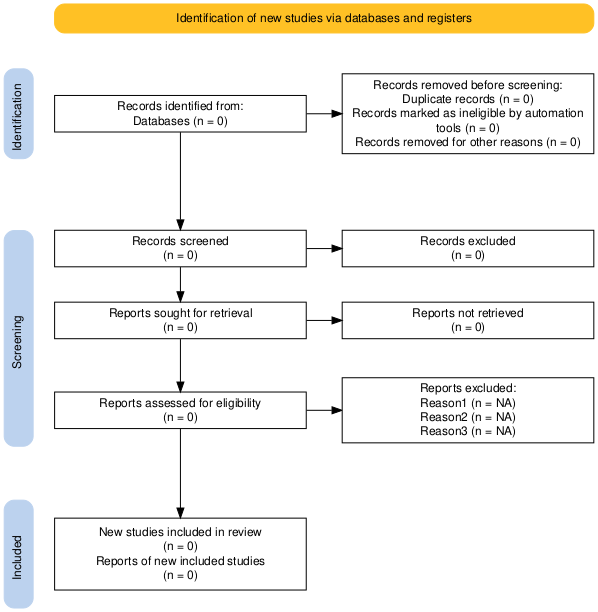
\includegraphics[width=\columnwidth]{prisma_flow.png}}
\caption{PRISMA flow diagram of the study selection process. Generated using the tool described in \cite{haddawayPRISMA2020PackageShiny2022}.}
\label{fig:prisma}
\end{figure}
% -----------------------------------------------------------------

Following the application of our PRISMA protocol and PICO selection criteria, a final corpus of [N] articles was retained for analysis (see Fig.~\ref{fig:prisma}). This section presents the results of this systematic review. 

We analyze this corpus according to the four main categories defined in our Data Extraction Grid (Table \ref{tab:grid}). Our analysis focuses on: (1) the model architectures employed, (2) the experimental frameworks and application domains, (3) the performance metrics used, and (4) the reported applicability and scalability of the proposed solutions. This structured analysis allows us to synthesize the current state-of-the-art and, most importantly, to identify the critical gaps that motivate our research.

\subsection{Analysis of Application Domains and Frameworks}
% Dans cette sous-section, vous analyserez les résultats de la Catégorie 2 de votre Grille d'Analyse (Tableau 2).
% Par exemple : "Our review shows that the primary application domain for ABM-MARL coupling is traffic simulation (N articles) and energy markets (N articles). 
% Applications to socio-ecological systems, particularly in agriculture or forestry, are notably rare (N articles)..."
% Vous parlerez aussi des plateformes (GAMA, NetLogo...) et de l'usage de données synthétiques vs. réelles.
In this subsection, we 

\subsection{Analysis of Model Architectures}
% C'est le cœur de votre analyse, basé sur la Catégorie 1.
% Par exemple : "The dominant MARL paradigm observed is Centralized Training with Decentralized Execution (CTDE), appearing in N\% of studies. 
% The most common algorithms are QMIX (N articles) and MADDPG (N articles)..."
% C'est ici que vous placez votre découverte clé :
% "...However, we found that hierarchical or hybrid architectures are critically under-explored, with only [X] studies 
% explicitly detailing such a design..."
In this subsection, we 

\subsection{Analysis of Performance and Applicability}
% C'est ici que vous analysez les Catégories 3 et 4.
% Par exemple : "A significant finding is that N\% of papers measure performance via algorithmic metrics (e.g., cumulative reward) 
% rather than system-level metrics (e.g., resource sustainability)..."
% Et votre deuxième lacune :
% "...Furthermore, we identified a critical gap regarding applicability: less than N\% of papers provide any data on computational cost 
% or training time, and formal scalability analysis (i.e., performance with a growing number of agents) is largely absent..."
In this subsection, we 

\section{Research Direction}

\textbf{RAJOUTER l'image de l'Architecture Fonctionnelle}

Our analysis of the recent literature reveals several structural trends. The strategic positioning of our doctoral research is articulated around these dynamics, which justify our focus on a hierarchical, constraint-based model.

First, the dominant paradigm for coordination in MARL is Centralized Training for Decentralized Execution (CTDE). This approach offers a pragmatic compromise: during the training phase, a centralized module leverages global information (observations and actions of all agents) to overcome non-stationarity and facilitate coordinated learning. During execution, each agent acts autonomously based solely on its local observations, which is a realistic constraint for distributed systems. The macro-decision-maker (RL) / micro-agent (ABM) architecture we propose can be interpreted as a sophisticated, structured instance of this CTDE paradigm.

Second, we observe a significant "Domain Maturity Gap" in MARL applications. Domains rooted in engineering, such as telecommunication networks, swarm robotics, or urban traffic control, are relatively advanced, with established benchmarks. In contrast, applications to complex Socio-Ecological Systems (SES)---particularly in agriculture, forestry, and land-use management---are more nascent and less standardized. This gap in applying advanced MARL to socio-ecological challenges represents a major research opportunity, which this work aims to address.

Furthermore, this domain gap exists partly because the scale and complexity of SES expose the limits of monolithic MARL architectures, where every entity is a complex learner. In response, hierarchical and hybrid models are gaining traction. These approaches combine one or more high-level (strategic) learning agents with low-level agents whose behavior is simpler (e.g., rule-based, heuristics, or cognitive architectures like BDI). This research direction is highly active as it directly addresses the need to reduce learning complexity and state-space dimensionality while maintaining behavioral plausibility.

Finally, we note a growing trend away from simple scalar reward maximization and towards constrained optimization. The "Safe RL" community is developing formal tools, such as Lagrangian optimization, to ensure agents avoid dangerous states. These concepts are directly translatable to sustainability challenges, where "avoiding a dangerous state" can be defined as "not depleting a critical resource" or "not exceeding a carbon emissions threshold." Similarly, questions of equity in the distribution of costs and benefits are becoming distinct optimization objectives.

These identified trends---the prevalence of CTDE, the nascent state of SES applications, the necessity of hierarchical models to manage complexity, and the move towards constrained optimization---form the central justification for the model proposed in our doctoral research. Our work is positioned at the intersection of these four active research frontiers.

\section{Conclusion}

\textbf{Rappeler la problematique et les obecjtifs de l'article}

\textbf{Quel a été la contribution de cet article?}

\textbf{Les limites et les travaux futures.}

In this paper, we conducted a systematic review of the literature at the intersection of Agent-Based Modeling and Multi-Agent Reinforcement Learning, guided by the PRISMA protocol. Our analysis revealed that while the field is active, its application to complex Socio-Ecological Systems remains nascent. We identified critical gaps in the dominant "full MARL" paradigm, namely a lack of scalability and a significant under-reporting of computational costs, which hinder practical application. In response, our analysis concludes that hierarchical and hybrid architectures, which combine high-level learning agents with simpler behavioral models, represent the most promising and scalable research direction. This approach, particularly when integrated with "Safe RL" concepts to enforce sustainability constraints, offers a viable pathway to developing the robust decision-support tools needed for real-world environmental management.

\section*{Acknowledgment}

The preferred spelling of the word ``acknowledgment'' in America is without 
an ``e'' after the ``g''. Avoid the stilted expression ``one of us (R. B. 
G.) thanks $\ldots$''. Instead, try ``R. B. G. thanks$\ldots$''. Put sponsor 
acknowledgments in the unnumbered footnote on the first page.


% Charge le guide de style IEEE (comment formater les refs)
\bibliographystyle{IEEEtran}

% Appelle votre base de données de citations
\bibliography{references}


\end{document}
